\documentclass[tikz,border=10pt]{standalone}
\usepackage{tikz}
\usetikzlibrary{positioning, shapes.multipart, arrows.meta}
\begin{document}

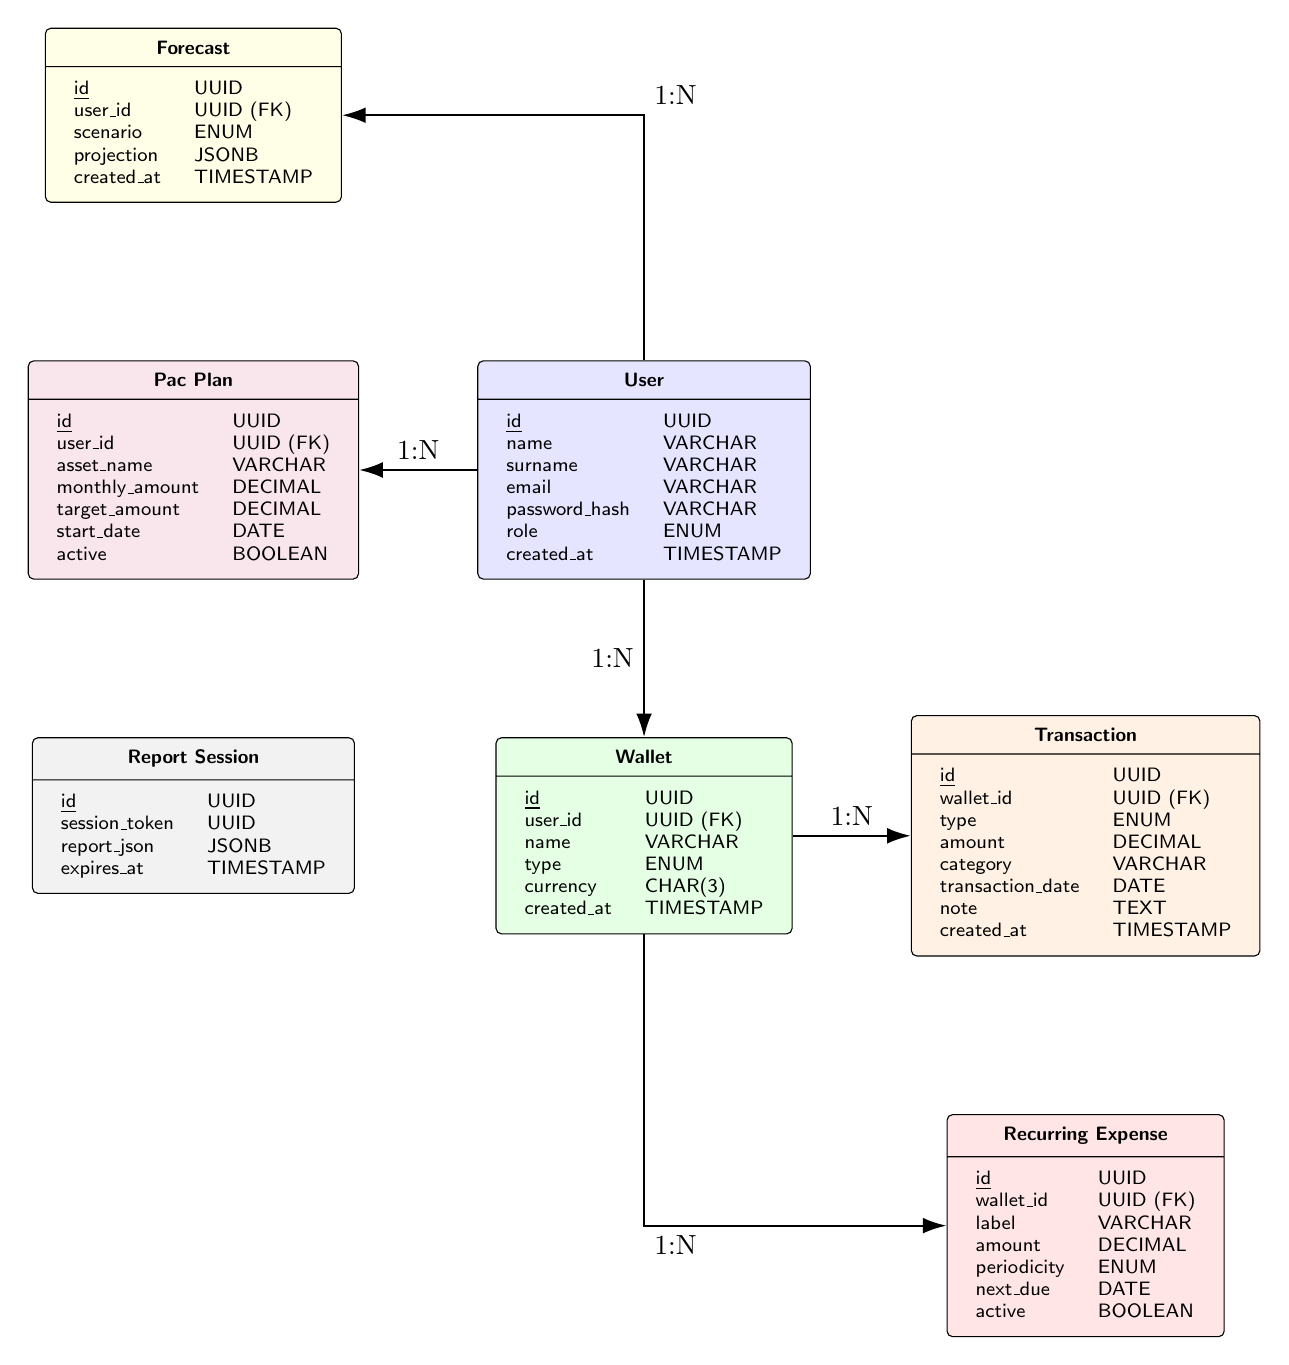
\begin{tikzpicture}[
    entity/.style={
        draw, rectangle split, rectangle split parts=2, 
        font=\sffamily\scriptsize, text centered, 
        inner sep=1ex, rounded corners=2pt,
        node distance=2cm and 1.5cm,
    },
    line/.style={draw, thick, -{Latex[length=3mm,width=2mm]}}
]

% Nodes
\node[entity, fill=blue!10] (user) {
    \textbf{User}
    \nodepart{two}
    \begin{tabular}{ll}
        \underline{id} & UUID \\
        name & VARCHAR \\
        surname & VARCHAR \\
        email & VARCHAR \\
        password\_hash & VARCHAR \\
        role & ENUM \\
        created\_at & TIMESTAMP
    \end{tabular}
};

\node[entity, fill=green!10, below=of user, node distance=2.5cm] (wallet) {
    \textbf{Wallet}
    \nodepart{two}
    \begin{tabular}{ll}
        \underline{id} & UUID \\
        user\_id & UUID (FK) \\
        name & VARCHAR \\
        type & ENUM \\
        currency & CHAR(3) \\
        created\_at & TIMESTAMP
    \end{tabular}
};

\node[entity, fill=purple!10, left=of user, node distance=1.5cm] (pac) {
    \textbf{Pac Plan}
    \nodepart{two}
    \begin{tabular}{ll}
        \underline{id} & UUID \\
        user\_id & UUID (FK) \\
        asset\_name & VARCHAR \\
        monthly\_amount & DECIMAL \\
        target\_amount & DECIMAL \\
        start\_date & DATE \\
        active & BOOLEAN
    \end{tabular}
};

\node[entity, fill=yellow!10, above=of pac, node distance=1cm] (forecast) {
    \textbf{Forecast}
    \nodepart{two}
    \begin{tabular}{ll}
        \underline{id} & UUID \\
        user\_id & UUID (FK) \\
        scenario & ENUM \\
        projection & JSONB \\
        created\_at & TIMESTAMP
    \end{tabular}
};

\node[entity, fill=gray!10, below=of pac, node distance=1cm] (reportsession) {
    \textbf{Report Session}
    \nodepart{two}
    \begin{tabular}{ll}
        \underline{id} & UUID \\
        session\_token & UUID \\
        report\_json & JSONB \\
        expires\_at & TIMESTAMP
    \end{tabular}
};

\node[entity, fill=orange!10, right=of wallet, node distance=1.5cm] (transaction) {
    \textbf{Transaction}
    \nodepart{two}
    \begin{tabular}{ll}
        \underline{id} & UUID \\
        wallet\_id & UUID (FK) \\
        type & ENUM \\
        amount & DECIMAL \\
        category & VARCHAR \\
        transaction\_date & DATE \\
        note & TEXT \\
        created\_at & TIMESTAMP
    \end{tabular}
};

\node[entity, fill=red!10, below=of transaction, node distance=1cm] (recexp) {
    \textbf{Recurring Expense}
    \nodepart{two}
    \begin{tabular}{ll}
        \underline{id} & UUID \\
        wallet\_id & UUID (FK) \\
        label & VARCHAR \\
        amount & DECIMAL \\
        periodicity & ENUM \\
        next\_due & DATE \\
        active & BOOLEAN
    \end{tabular}
};

% Edges
\draw[line] (user) -- node[left] {1:N} (wallet);
\draw[line] (user) -- node[above] {1:N} (pac);
\draw[line] (user) |- node[above right] {1:N} (forecast);
\draw[line] (wallet) -- node[above] {1:N} (transaction);
\draw[line] (wallet) |- node[below right] {1:N} (recexp);

\end{tikzpicture}
\end{document}
